\documentclass[11pt]{article}
\addtolength{\oddsidemargin}{-1.cm}
\addtolength{\textwidth}{2cm}
\addtolength{\topmargin}{-2cm}
\addtolength{\textheight}{3.5cm}
\newcommand\tab[1][1cm]{\hspace*{#1}}
\usepackage[pdftex]{graphicx}
\usepackage{pdflscape}
\usepackage[T1]{fontenc}
\usepackage{hyperref}
\usepackage{float}
\usepackage{cite}
\usepackage{todonotes}

\hypersetup{
	colorlinks=true,
	linkcolor=black,
	filecolor=magenta,
	urlcolor=cyan,
}

% define the title
\author{Binary Ninjaz}
\title{Harvest}
\begin{document}
\begin{titlepage}

	\begin{center}
		% Upper part of the page
		\textsc{\LARGE Binary Ninjaz}\\[0.3cm]
		% Title
		\rule{\linewidth}{0.5mm} \\[0.5cm]
		{ \huge \bfseries Harvest \\
		  \vspace{0.3cm}\large \bfseries User Manual}\\[0.5cm]
		\rule{\linewidth}{0.5mm} \\[1cm]


		\begin{minipage}{0.4\textwidth}
			\begin{flushleft} \large
				\emph{} \\
				Letanyan {Arumugam}
			\end{flushleft}
		\end{minipage}
		\begin{minipage}{0.4\textwidth}
			\begin{flushright} \large
				\emph{} \\
				14228123
			\end{flushright}
		\end{minipage}

		\begin{minipage}{0.4\textwidth}
			\begin{flushleft} \large
            	\emph{} \\
				Sizo {Duma}
			\end{flushleft}
		\end{minipage}
		\begin{minipage}{0.4\textwidth}
			\begin{flushright} \large
				\emph{} \\
				15245579
			\end{flushright}
		\end{minipage}

		\begin{minipage}{0.4\textwidth}
			\begin{flushleft} \large
				\emph{} \\
				Teboho {Mokoena}
			\end{flushleft}
		\end{minipage}
		\begin{minipage}{0.4\textwidth}
			\begin{flushright} \large
				\emph{} \\
				14415888
			\end{flushright}
		\end{minipage}

		\begin{minipage}{0.4\textwidth}
			\begin{flushleft} \large
				\emph{} \\
				John {Ojo}
			\end{flushleft}
		\end{minipage}
		\begin{minipage}{0.4\textwidth}
			\begin{flushright} \large
				\emph{} \\
				15096794
			\end{flushright}
		\end{minipage}

        \begin{minipage}{0.4\textwidth}
			\begin{flushleft} \large
				\emph{} \\
				Kevin {Reid}
			\end{flushleft}
		\end{minipage}
		\begin{minipage}{0.4\textwidth}
			\begin{flushright} \large
				\emph{} \\
				15008739
			\end{flushright}
		\end{minipage}

        \begin{minipage}{0.4\textwidth}
			\begin{flushleft} \large
				\emph{} \\
				Shaun {Yates}
			\end{flushleft}
		\end{minipage}
		\begin{minipage}{0.4\textwidth}
			\begin{flushright} \large
				\emph{} \\
				16007493
			\end{flushright}
		\end{minipage}

		\vspace{1cm}
		\rule{\linewidth}{0.5mm} \\[1cm]
		\textsc{\Large Stakeholders}\\[1cm]

		\begin{minipage}{0.4\textwidth}
			\begin{flushleft} \large
				\emph{} \\
				SAMAC:
			\end{flushleft}
		\end{minipage}
		\begin{minipage}{0.4\textwidth}
			\begin{flushright} \large
				\emph{} \\
				Barry Christie
			\end{flushright}
		\end{minipage}


	\end{center}
\end{titlepage}

\newpage
\pagenumbering{Roman}
\tableofcontents
\newpage
\listoffigures

\newpage
\pagenumbering{arabic}

\newpage
\section{System Overview}

\subsection{Purpose}
The need for this system is due to the fact current yield tracking and measuring worker performance is done manually and on paper. This allows for a more efficient way of carrying out that process. This more efficient process will help farmers better track and manage produce collection. Finding cold spots and irregularities in orchards or by workers.

\subsection{Project Scope}
The goal of the project, Harvest, is a system to assist growers with yield data and optimise worker performance. The aim of the project is to produce a system that can efficiently measure the amount of work done by a worker, track the foremen on a farm, record information and data, and display the necessary information.

\subsection{Definitions}
\begin{itemize}
\item Farmer - The lead manager of a farm.
\item Foreman - Overseer of work done by workers in the field.
\item Worker - Labourer that collects produce from the farm lands.
\item Farm - A collection of orchards with a similar crop.
\item Orchard - An area allocated by the farmer for where produce may be collected.
\item Collections - Produce collected by workers on a farm.
\item Entity - Either a farm, orchard, worker or foreman.
\item Session - The period when foremen will be tracking workers collecting produce.
\end{itemize}
\todo{more definitions?}

\newpage
\subsection{UML Domain Model}
\todo{Use domain model not class diagram}
\begin{figure}
 \centering
 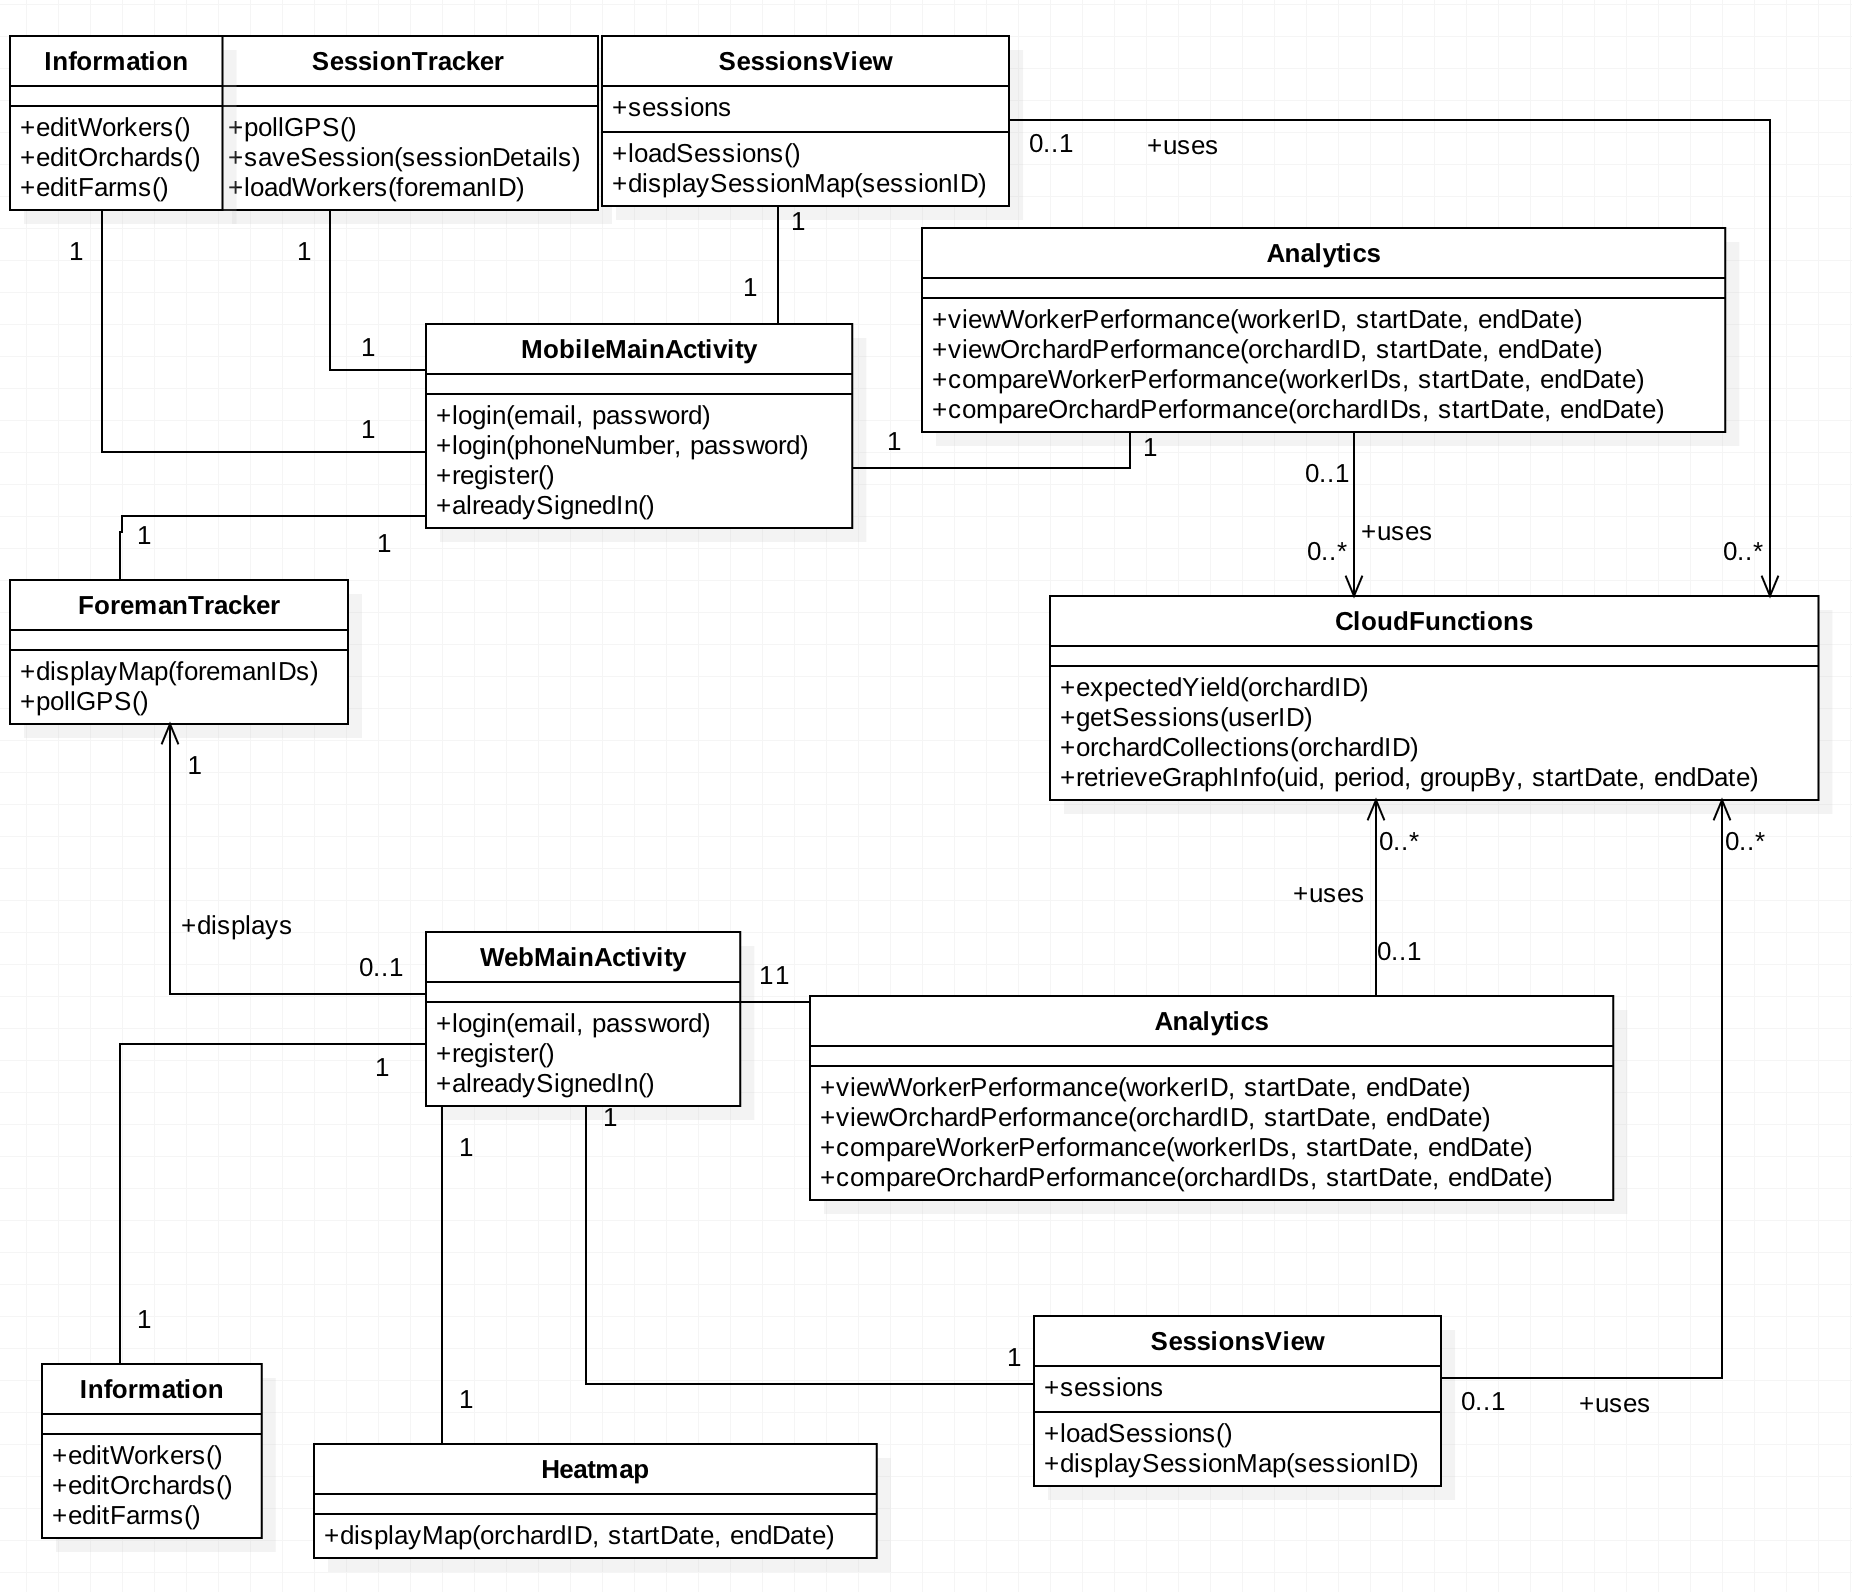
\includegraphics[width=12cm, keepaspectratio]{UMLClassDiag.png}
 \caption{Domain Model}
 \label{DomainModel}
\end{figure}

\section{Functional Requirements:}
\subsection{Users}
\subsubsection{Farmers}
Farmers will be the main beneficiary for using the system. Information about what data is collected and analysis on said collected data is provided. Managing administrative details is possible however not the main focus. It is rather for helping the system provide more specific insights into where and how collections are made. The system produces graphs, heatmaps and summaries of work done by entities. It is on the farmer to critque the data to find where performance can be improved or work may need fixing.

\subsubsection{Foremen}
Foremen will use the system to track how much each worker collects. The system will log where and when the user logs a collection. Foremen simply need to tap on button next to a workers name when said worker collects a bag of produce.

\subsection{Subsystems}
\begin{itemize}
\item Database - Stores information such as entity details and collection data.
\item Location Services - Manages location information regarding foremens mobile devices.
\item Cloud Functions - A helper service that runs intensive computation on servers where the databse is stored.
\item Mobile Application - The mobile device application used in field.
\item Website - A web based interface to interact with the system.
\end{itemize}
See \ref{ComponentDiagram} for diagram representation.
\begin{figure}
 \centering
 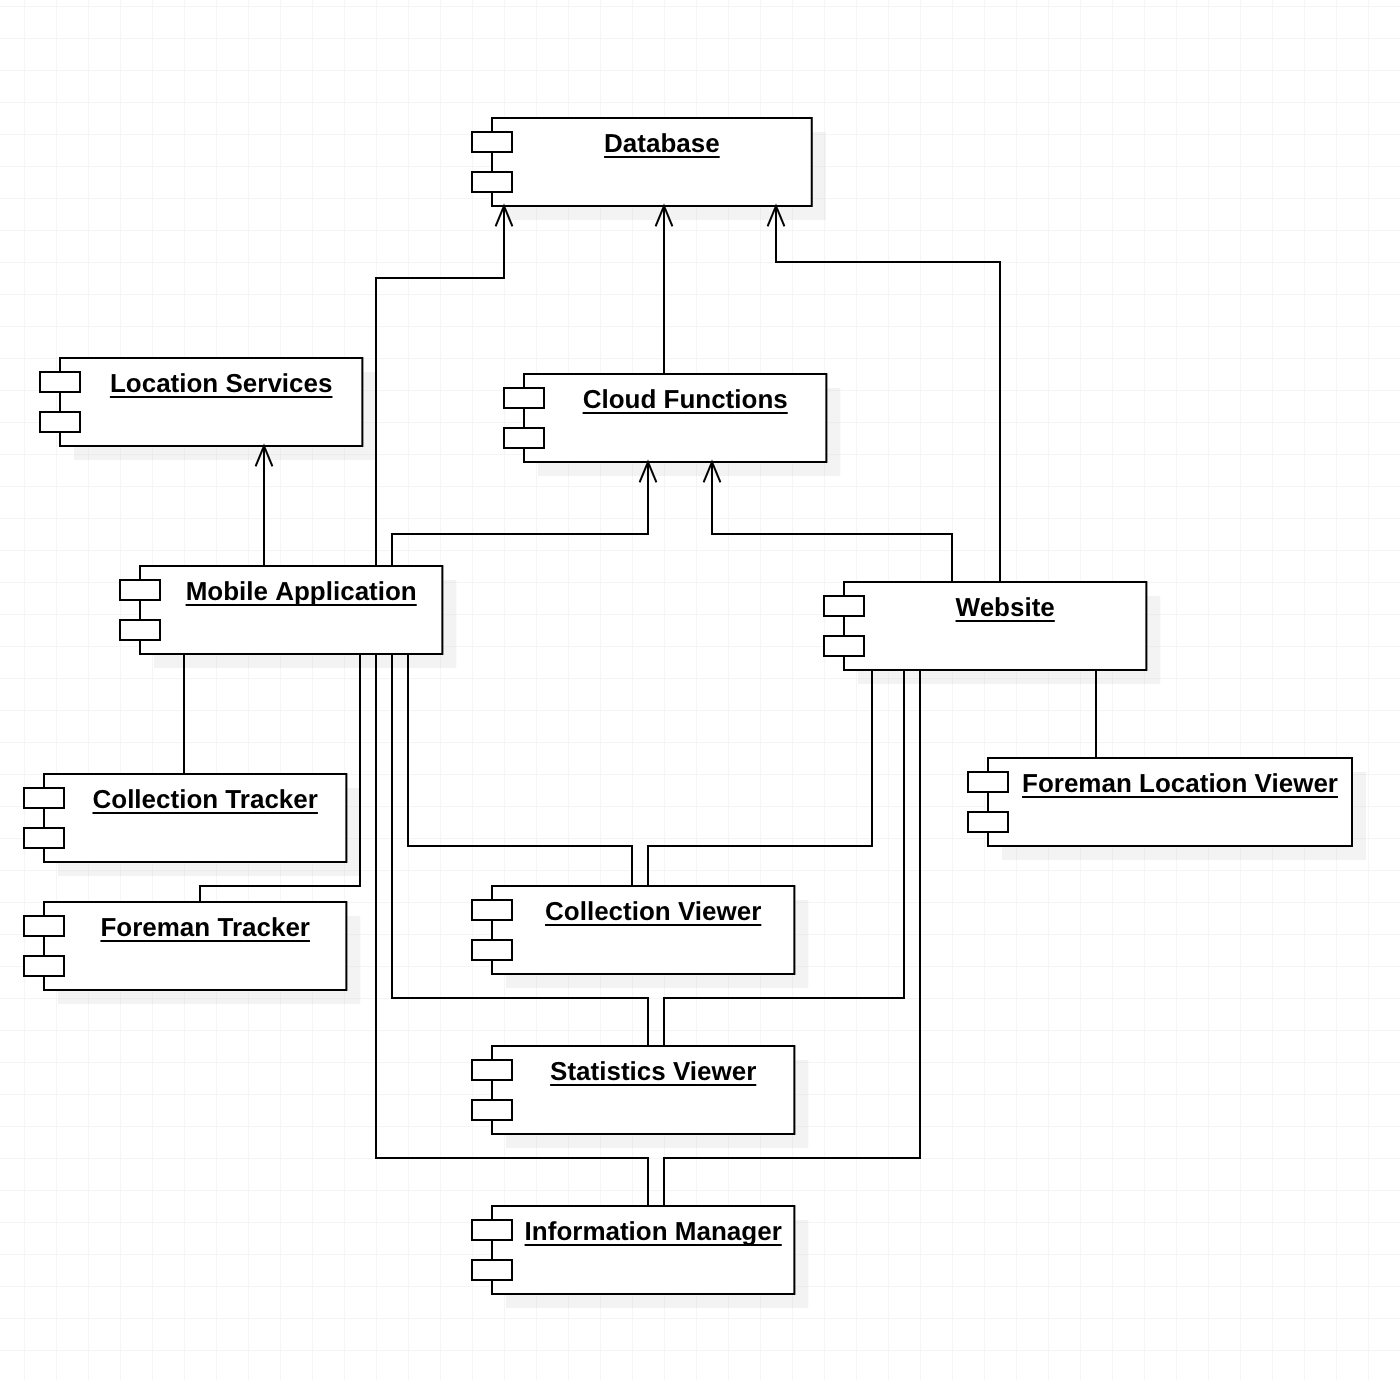
\includegraphics[width=12cm, keepaspectratio]{ComponentDiagram.png}
 \caption{Component Diagram}
 \label{ComponentDiagram}
\end{figure}

\subsection{Specific Requirements}
\begin{itemize}
  \item On sign in Harvest shall verify credentials against the database before signing them in.
  \item Harvest shall create a profile on the database for the user through a registration form.
  \item Harvest shall measure yield through the input view of the mobile interface.
  \item The Harvest mobile interface shall make use of GPS data and based on weight and location assumptions, it must give approximate yield estimates not only for each orchard, but for each approximate location where the data was entered.
  \item The Harvest system shall make use of analytics to measure worker performance.
  \item The Harvest website shall display heat map data, showing the locations in which the most yield has been collected.
  \item The Web interface shall show detailed information about produce. (e.g. cultivar, year planted).
  \item The Harvest system shall do administrative tasks through the web interface.
  \item The Harvest website shall give the farmer/administrator a real time map view of the foreman's location.
  \item Both foremen and farmers shall have access to the mobile interface, with foremen unable to carry out any administrative changes or view analytical data on it.
  \item Only farmers shall make use of the website, as it is designed to track their workers, foremen and measure performance in and around their farms.
\end{itemize}

\section{Non-functional Requirements}

\subsection{Conservative Battery Usage}

\subsubsection{Why?}
Foremen will be expected to use the mobile application throughout a session, which may last multiple hours. If mobile devices were to be running out of battery before the end of session the services will not be able to produce accurate productivity measurements and statistics.

\subsubsection{How?}
Reducing location accuracy might not provide the most accurate results. The battery savings are more important than having perfect accuracy. Network transactions will also be limited to only a few calls only when neccessary. Heavy usage of cache storage will be employed. Calls requested data changes will be made and requests to only download new data and changes will be download instead of full re-downloads of data.

\subsection{Intuitive User Interface}

\subsubsection{Why?}
The target audience of the system are people who care about doing their work and not about learning a new systems.

\subsubsection{How?}
We intend to use the design languages that are well established on the platforms that the user facing experience will be displayed on. Following design guidelines set by Apple \footnote{\url{https://developer.apple.com/design/human-interface-guidelines/ios/overview/themes/}} and by Google Android \footnote{\url{https://material.io/design/}}.

\subsection{Smooth User Experience}

\subsubsection{Why?}
Having an experience that requires a steep learning curve or has sharp edges will quickly lead to people reverting back to an old system. Even if the old system has the same sharp edges their known about and users are used to it. Hence to make sure users move away from their old system of completing their tasks, we must provide as smooth a transition as possible.

\subsubsection{How?}
The video game industry has faced this problem since their inception. We will look to game designer to see how they have solved their problem of introducing and teaching concepts to their players seamlessly. One such example is tutorial systems, where to introduce a new concept, the user is faced with a problem that has one and only one obvious solution. We will employ this technique in our implementation of the system.

\section{System Architecture}
\subsection{Determining Design Objectives}
\begin{itemize}
\item The design is aimed to provide accessibility, data integrity and optimize performance.
\item The design is also aimed at producing a user friendly easy to use system.
\item The design is aimed at easing facilitation and automation of work.
\end{itemize}

\subsection{Interfaces}

\subsubsection{User Interfaces:}
\begin{itemize}
\item Mobile Application Interface
	\begin{itemize}
	\item Authentication Screen: Provides a way for farmers and foremen to sign into the system. Foremen will sign in using a mobile phone number sign in. Foreman sign in will produce a different view which will only show the yield collector. Farmer sign in will show all options available.
	\item Yield Collector: Track the work done by each worker during a session.
	\item Information: Manage information about entities.
	\item Sessions: View raw session data. Such as time started and ended, where and when pick ups were made.
	\item Stats: View graphs about over periods of time regarding entity comparison differences.
	\item Settings: Manage certain settings such as login details. View help about the system is also provided.
	\end{itemize}
\item Web Page Interface
	\begin{itemize}
	\item Authentication Screen: Provides a way for farmers to sign into the system.
	\item Foreman Tracker: Track where foremen currently are during a session.
	\item Information: Manage information about entities.
	\item Sessions: View raw session data. Such as time started and ended, where and when pick ups were made.
	\item Stats: View graphs about over periods of time regarding entity comparison differences.
	\item Settings: Manage certain settings such as login details. View help about the system is also provided.
	\end{itemize}
\end{itemize}
% 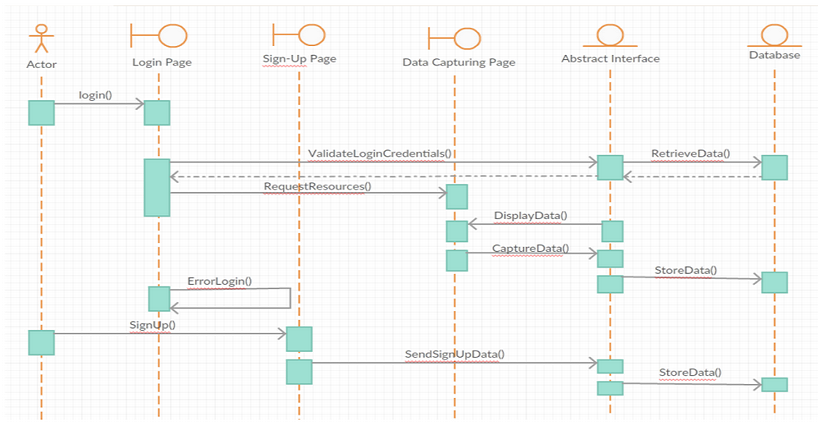
\includegraphics[width=1.2\linewidth]{sequenceDiag.PNG}

\subsubsection{Hardware Interfaces:}
Most hardware interaction aside from basic usage will be with GPS systems found on mobile devices. The system will use GPS data provided by mobile devices to tag collection data and track foremen during sessions.

\subsubsection{Software Interfaces:}
\begin{itemize}
\item Firebase Realtime Database: The system interacts with the database using firebase API on Swift, Java and Javascript. This interaction is simple for storage and retrieval of JSON data.
\item Google Maps SDK: To provide map data we use the SDK provided by Google for Swift, Java and Javascript. The SDK is used for map image data. Map overlays provided by the SDK are also used. Overlays such as heat-maps, markers and polygons are used to provide a more complete user experience.
\end{itemize}

\subsection{Architectural Styles}
The architectural structural design of our the Harvest system is a Persistence Framework. The system has 3 main subsystems (Android Application, IOS Application and the website) all heavily reliant on the database system providing them with efficient object storage and retrieval without the need for implementation detail. It also hides the database details such as implementation from the subsystems, and  therefore uses an abstract interface to manipulate data.


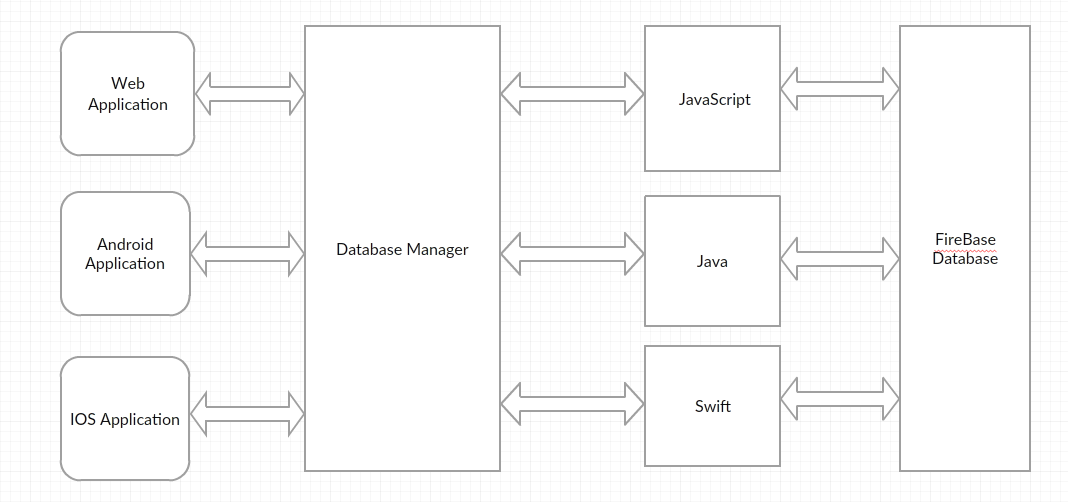
\includegraphics[width=1.0\linewidth]{persistenceFrameWork.PNG}

\subsubsection{Reviewing the Architectural Design}
\begin{itemize}
\item[$\bullet$]The Harvest application is accessible from a smartphone/tablet/desktop computer.
\item[$\bullet$]The Harvest system checks whether the user is registered before signing them in.
\item[$\bullet$]Harvest creates a new profile of the user when registering them.
\item[$\bullet$]Harvest measures yield through the input view of the mobile interface.
\item[$\bullet$]Harvest does facilitate GPS data filtering and Web Functionality.
\item[$\bullet$]The software application does facilitate the idea of tracking.
\end{itemize}

\subsection{System Configuration}
\subsubsection{Technology Used}
\begin{itemize}
\item[$\bullet$]Database System : Firebase
\item[$\bullet$]IDE's: Xcode, Android studio
\item[$\bullet$]Programming languages: XML (Android UI); Java (Android Backend); Swift (IOS); HTML, CSS, JavaScript (Website)
\end{itemize}

\subsubsection{Deployment Diagram}
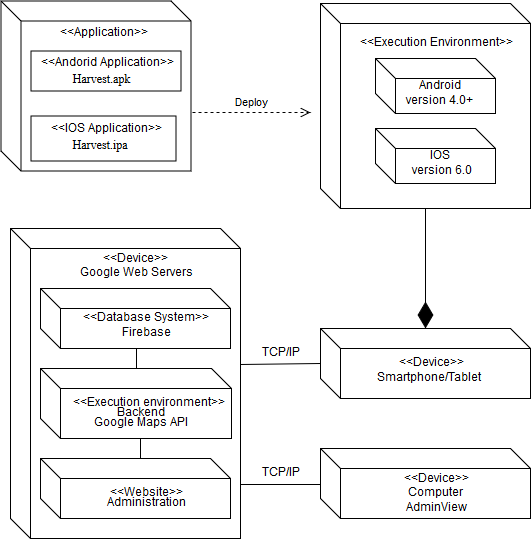
\includegraphics[width=.85\linewidth]{deployment.png}


\end{document}
